% https://www-igm.univ-mlv.fr/~lecroq/string/node14.html

\section*{Algoritmo de Boyer-Moore}
\phantomsection
\addcontentsline{toc}{section}{Algoritmo de Boyer-Moore}

\phantomsection
\subsection*{Introducción del Algoritmo de Boyer-Moore}
% \addcontentsline{toc}{subsection}{Introducción del Algoritmo de Boyer-Moore}

El algoritmo de Boyer-Moore realiza su búsqueda escaneando el patrón deseado desde la posición derecha hasta la posición izquierda. Este utiliza dos heurísticas para completar su cometido, llamadas ‘Bad Character Rule’ y ‘Good Suffix Rule’.
Para ambas heurísticas el algoritmo realiza un “preprocesamiento” del patrón, donde se elaboran dos tablas de interés:
\begin{itemize}
    \item La tabla BC (Bad Character) basa su elaboración en el desplazamiento necesario para ir desde el carácter que se encuentra más a la derecha (del patrón) hasta la primera ocurrencia de los caracteres específicos que lo componen. Si 
    \item La GS (Good Suffix) se elabora a partir de las coincidencias encontradas entre los sufijos del patrón y los caracteres restantes. Nos da el desplazamiento necesario, desde la izquierda, para encontrar dichas coincidencias. Estas pueden ser exactas (el prefijo aparece exactamente igual) o aproximadas (aparece una parte del sufijo).
\end{itemize}

Cuando el algoritmo va realizando las comparaciones entre el patrón y el texto y encuentre una discordancia, la decisión entre usar el desplazamiento recomendado por la tabla BC o la tabla GS dependerá netamente de cual de las dos le ofrezca un mayor “salto” o ventaja.

\phantomsection
\subsection*{Implementación del Algoritmo de Boyer-Moore}
% \addcontentsline{toc}{subsection}{Implementación del Algoritmo de boyer-Moore}
(Con ayuda de \cite{boyer-moor_algorithm_1997}, \cite{101145359842359859}, \cite{gusfield_1997}, \cite{exactOnline} y \cite{pdfBoyer})

\begin{algorithm} [H]
    \caption{Algoritmo de Boyer\_Moore}\label{alg:BM}
    \begin{algorithmic} [1]
        \Procedure{Boyer-Moore}{(patron, texto)}
            \State $sizeP = len(P)$
            \State $sizeT = len(T)$
            \State $boyerMooreBadChar = [0] * 256$ \Comment{256 es el número generalmente aceptado como alfabéto}
            \For{$0 \leq i < sizeP-1$}
                \State $boyerMooreBadChar[ord(patron[i])] = sizeP - i - 1$
            \EndFor
            
            \State $suff = [0] * sizeP$
            \State $f = 0$
            \State $g = sizeP -1$
            \State $suff[sizeP -1] = sizeP$
            \For{$sizeP -2 \geq i > -1$}
                \If{$i > g \land suff[i + sizeP -1 - f] < i - g$}
                    \State $suff[i] = suff[i + sizeP -1 -f]$
                \Else
                    \If{$i < g$}
                        \State $g = i$
                    \EndIf
                    \State $f = i$
                    \While{$g \geq 0 \land P[g] == P[g + sizeP - 1 - f]$}
                        \State $g -= 1$
                    \EndWhile
                    \State $suff[i] = f - g$
                \EndIf
            \EndFor

            \State $boyerMooreGoodSuffix = [sizeP] * sizeP$
            \For{$0 \leq i < sizeP$}
                \If{$suff[i] == i + 1$}
                    \For{$0 \leq j < sizeP - 1 - i$}
                        \If{$boyerMooreGoodSuffix[j] == sizeP$}
                            \State $boyerMooreGoodSuffix[j] = sizeP - 1 - i$
                        \EndIf
                    \EndFor
                \EndIf
            \EndFor
            \For{$0 \leq i < sizeP-1$}
                \State $boyerMooreGoodSuffix[sizeP - 1 - suff[i]] = sizeP - 1 - i$
            \EndFor

            \State $i = 0$
            \algstore{bm}
    \end{algorithmic}
\end{algorithm}

\begin{algorithm} [H]
    \begin{algorithmic} [1]
        \algrestore{bm}
                \State $j = 0$

                \While{$j \leq sizeT - sizeP$}
                \State $i = sizeP - 1$
                \While{$i != -1 \land patron[i] == texto[i+j]$}
                    \State $i -= 1$
                \EndWhile
                \If{$i < 0$}
                    \State $print(j)$
                    \State $j += boyerMooreGoodSuffix[0]$
                \Else
                    \State $j += max(boyerMooreGoodSuffix[i], boyerMooreBadChar[ord(T[i+j])] - sizeP + 1 + i)$
                \EndIf
            \EndWhile
        \EndProcedure
    \end{algorithmic}
\end{algorithm}


\phantomsection
\subsection*{Análisis del Algoritmo de Boyer-Moore}
% \addcontentsline{toc}{subsection}{Análisis del Algoritmo de Boyer-Moore}

\subsubsection*{Paso 1: Establecer el tamaño n de los datos}
% \addcontentsline{toc}{subsubsection}{Paso 1: Establecer el tamaño n de los datos}
El tamaño de los datos esta dado por m + n (Siendo ‘m’ el tamaño del texto y ‘n’ el tamaño del patrón)

\subsubsection*{Paso 2: Determinar las operaciones de interés}
% \addcontentsline{toc}{subsubsection}{Paso 2: Determinar las operaciones de interés}
Las operaciones van a variar dependiendo del módulo. Principalmente, utilizaremos de referencia aquellas relacionadas a comparaciones (‘==’, ¡‘!=’) y asignaciones (‘=’)

\subsubsection*{Paso 3: Encontrar los casos base}
% \addcontentsline{toc}{subsubsection}{Paso 3}
Dividiremos esta sección en Preprocesamiento y Búsqueda, de la forma:
\begin{itemize}
    \item Preprocesamiento
    \begin{itemize}
        \item Heurística de caracteres malos ($w$ es el tamaño del alfabeto)
        \[T_{HCM}(0) = w \hskip1cm \texttt{si } n = 0\]
        \[T_{HCM}(n) = 1 + T_{HCM}(n-1) \hskip1cm \texttt{si } n > 0\]
        \item Herística de sufijos buenos
        \[T_{HSB}(0) = 0 \hskip1cm \texttt{si } n \leq 1\]
        \[T_{HSB}(n) = 1 + (n-1) + T_{HSB}(n-1) \hskip1cm \texttt{si } n > 1\]
    \end{itemize}
    \item Búsqueda
    \[T_{patrón}(0) =  0\]
    \[T_{patrón}(1) = 1\]

    \[T_{patrón}(n) = 1 + T_{patrón}(n-1)\]

    \[T_{texto}(0) =  0\]
    \[T_{texto}(1) = 1\]

    \[T_{texto}(m) = 1 + T_{texto}(m-1)\]
    \[T_{Búsqueda}(n,m) = T_{patrón}(n) * T_{texto}(m)\]
\end{itemize}
Eso entonces se junta para que la ecuación de tiempo del Boyer-Moore de:
\[T_{Boyer-Moore}(m,n) = T_{HCM}(n) + T_{HSB}(n) + T_{Búsqueda}(n,m)\]

\subsubsection*{Paso 4: Evaluando la ecuación recursiva}
% \addcontentsline{toc}{subsubsection}{Paso 4}
\begin{itemize}
    \item Preprocesamiento
    \begin{itemize}
        \item Heurística de caracteres malos
        \[T_{HCM}(n) = 1 + 1+ 1+ ... + 1 + w\]
        \[T_{HCM}(n) = n + w\]
        \item Heurística de sufijos buenos
        \[T_{HSB}(n) = 1 +  (n-1) + 1 + (n-2) + 1 + (n-3) ... + 0\]
        \[T_{HSB}(n) = n + (n-1) + (n-2) + (n-3) ... + 0\]
        \[T_{HSB}(n) = \frac{n*(n+1)}{2} = \frac{n^2 + n}{2}\]
    \end{itemize}
    \item Búsqueda
    \[T_{patrón}(n) = 1 + 1 + 1 + 1 ... + 1 + 1\]

    \[T_{patrón}(n) = n \]

    \[T_{texto}(m) = 1 + 1 + 1 + 1 ... + 1 + 1\]

    \[T_{texto}(m) = m \]
    \[T_{Búsqueda}(n,m) = n * m\]
\end{itemize}

\[T_{Boyer-Moore}(n,m) = (n+w) + (\frac{n^2 + n}{2}) + n*m\]

\subsubsection*{Paso 5: O-grande}
% \addcontentsline{toc}{subsubsection}{Paso 5}
Dado a los pasos anteriores podemos concluir que el O-grande de Boyer-Moore es $O(w) + O(n^2) + O(n*m) \sim O(n*m)$
Es importante destacar que aunque en el peor de los casos es $n*m$, pero que es considerado el más eficiente de los 4 porque el O-grande normal es $O(\frac{n}{m})$ como lo describen \cite{TwoWaySM}

\subsubsection*{Paso 6}
% \addcontentsline{toc}{subsubsection}{Paso 6}
\begin{figure} [H]
    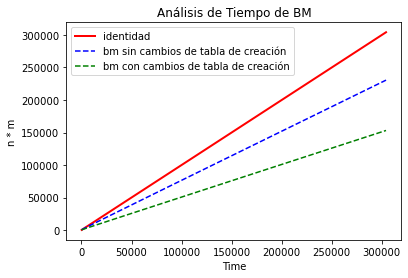
\includegraphics[width=0.5\textwidth]{../codigoPythonJupyter/bm/Final.png}
    \caption{Boyer-Moore (Apéndice boyermoore.ipynb)}
    \label{fig:bm}
\end{figure}
Este generamos dos porque en proceso de hacer pruebas nos percatamos que la generación de las tablas al ser uno o la otra no tenían que contarse todo el tiempo y creamos un if para que generara la más rápida.

% TODO
% http://doi.acm.org/10.1145/2431211.2431212
% https://www.cs.utexas.edu/users/moore/publications/fstrpos.pdf 